\documentclass[11pt,letterpaper]{article}
\usepackage[lmargin=1in,rmargin=1in,tmargin=1in,bmargin=1in]{geometry}
\usepackage{../style/homework}
\usepackage{../style/commands}
\setbool{quotetype}{true} % True: Side; False: Under
\setbool{hideans}{false} % Student: True; Instructor: False

% -------------------
% Content
% -------------------
\begin{document}

\homework{6: Due 10/08}{I'm fine. It's just that life is pointless and nothing matters and I'm always tired.}{Andy Dwyer, Parks and Recreation}


% Problem 1
\problem{10} Plot the function $f(x):= 4 - 3x$, being as accurate as possible. 
	\[
	\fbox{
	\begin{tikzpicture}[scale=2,every node/.style={scale=0.5}]
	\begin{axis}[
	grid=both,
	axis lines=middle,
	ticklabel style={fill=blue!5!white},
	xmin= -7, xmax=7,
	ymin= -6.5, ymax=6.5,
	xtick={-6,-4,-2,0,2,4,6},
	ytick={-6,-4,-2,0,2,4,6},
	minor tick = {-5,-3,...,5},
	xlabel=\(x\),ylabel=\(y\),
	]
	\addplot[thick, domain= -7:7] {4 - 3*x};
	\addplot[soldot,mark size=1.5pt] coordinates{(-4,16)(-3,13)(-2,10)(-1,7)(0,4)(1,1)(2,-2)(3,-5)(4,-8)};
	\end{axis}
	\end{tikzpicture}
	}
	\] \pspace

\sol To sketch the line, we should find around 8--12 equally spaces points on the curve and connect them ``smoothly.''
	\begin{table}[!ht]
	\centering
	\begin{tabular}{r||rrrrrrrrrr}
	$x$ & $-4$ & $-3$ & $-2$ & $-1$ & $0$ & $1$ & $2$ & $3$ & $4$ \\ \hline
	$f(x)$ & $16$ & $13$ & $10$ & $7$ & $4$ & $1$ & $-2$ & $-5$ & $-8$
	\end{tabular}
	\end{table}





\newpage





% Problem 2
\problem{10} Plot the function $f(x):= x^2 + 4x - 1$, being as accurate as possible. 
	\[
	\fbox{
	\begin{tikzpicture}[scale=2,every node/.style={scale=0.5}]
	\begin{axis}[
	grid=both,
	axis lines=middle,
	ticklabel style={fill=blue!5!white},
	xmin= -7, xmax=7,
	ymin= -6.5, ymax=6.5,
	xtick={-6,-4,-2,0,2,4,6},
	ytick={-6,-4,-2,0,2,4,6},
	minor tick = {-5,-3,...,5},
	xlabel=\(x\),ylabel=\(y\),
	]
	\addplot[samples=100,thick, domain= -7:7] {x^2 + 4*x - 1};
	\addplot[soldot,mark size=1.5pt] coordinates{(-5,4)(-4,-1)(-3,-4)(-2,-5)(-1,-4)(0,-1)(1,4)(2,11)(3,20)(4,41)};
	\end{axis}
	\end{tikzpicture}
	}
	\] \pspace

\sol To sketch the line, we should find around 8--12 equally spaces points on the curve and connect them ``smoothly.''
	\begin{table}[!ht]
	\centering
	\begin{tabular}{r||rrrrrrrrrrr}
	$x$ & $-5$ & $-4$ & $-3$ & $-2$ & $-1$ & $0$ & $1$ & $2$ & $3$ & $4$ \\ \hline
	$f(x)$ & $4$ & $-1$ & $-4$ & $-5$ & $-4$ & $-1$ & $4$ & $11$ & $20$ & $41$
	\end{tabular}
	\end{table}




% Problem 3
\problem{10} Plot the function $f(x):= \dfrac{x + 1}{x^2 + 1}$, being as accurate as possible. 
	\[
	\fbox{
	\begin{tikzpicture}[scale=2,every node/.style={scale=0.5}]
	\begin{axis}[
	grid=both,
	axis lines=middle,
	ticklabel style={fill=blue!5!white},
	xmin= -7, xmax=7,
	ymin= -6.5, ymax=6.5,
	xtick={-6,-4,-2,0,2,4,6},
	ytick={-6,-4,-2,0,2,4,6},
	minor tick = {-5,-3,...,5},
	xlabel=\(x\),ylabel=\(y\),
	]
	\addplot[samples=100,thick, domain= -7:7] {(x+1)/(x^2+1)};
	\addplot[soldot,mark size=1.5pt] coordinates{(-5,-2/13)(-4,-3/17)(-3,-1/5)(-2,-1/5)(-1,0)(0,1)(1,1)(2,3/5)(3,2/5)(4,5/17)(5,3/13)};
	\end{axis}
	\end{tikzpicture}
	}
	\] \pspace

\sol To sketch the line, we should find around 8--12 equally spaces points on the curve and connect them ``smoothly.''
	\begin{table}[!ht]
	\centering
	\begin{tabular}{r||rrrrrrrrrrrr}
	$x$ & $-5$ & $-4$ & $-3$ & $-2$ & $-1$ & $0$ & $1$ & $2$ & $3$ & $4$ & 5 \\ \hline
	$f(x)$ & $-\frac{2}{13}$ & $-\frac{3}{17}$ & $-\frac{1}{5}$ & $-\frac{1}{5}$ & $0$ & $1$ & $1$ & $\frac{3}{5}$ & $\frac{2}{5}$ & $\frac{5}{17}$ & $\frac{3}{13}$
	\end{tabular}
	\end{table}





\newpage





% Problem 4
\problem{10} Let $f(x):= 5x - 3$.
\begin{enumerate}[(a)]
\item Find $f(1)$. \pvspace{1.3cm}
	\[
	f(1)= 5(1) - 3= 5 - 3= 2
	\] \pvspace{2.1cm}


\item What value(s) for $x$ make the output of $f(x)$ twice the output from (a)? \pspace

{\itshape The output from (a) was 2. So twice this would be 4. We want $x$ so that $f(x)= 4$. But then 
	\[
	\begin{aligned}
	5x - 3&= 4 \\
	5x&= 7 \\
	x&= \frac{7}{3}
	\end{aligned}
	\]
} \pvspace{0.7cm}


\item Is $(1, 2)$ on the graph of $f(x)$? Explain. \pspace

{\itshape We have $f(1)= 5(1) - 3= 5 - 3= 2$ so that $(1, 2)$ is a point on the graph. But this is exactly the given point. Alternatively, because $y= 5x - 3$, we check $2 \stackrel{?}{=} 5(1) - 3= 2$ so that $(1, 2)$ is on the graph of $f(x)$.} \pvspace{2.5cm}


\item Is $(3, 5)$ on the graph of $f(x)$? Explain. \pspace

{\itshape We have $f(3)= 5(3) - 3= 15 - 3= 12$ so that $(3, 12)$ is a point on the graph. But this is not the point $(3, 5)$. Therefore, $(3, 5)$ is not a point on the graph of $f(x)$. Alternatively, because $y= 5x - 3$, we check $5 \stackrel{?}{=} 5(3) - 3= 12$, which is false so that $(3, 5)$ is not on the graph of $f(x)$.}
\end{enumerate}





\newpage





% Problem 5
\problem{10} Define the following functions:
	\[
	\begin{aligned}
	f(x)&:= x^3 - x \\
	g(x)&:= x^2 - 2x + 3 \\
	h(x)&:= x^4 + x^2
	\end{aligned}
	\]
Determine if the functions $f(x)$, $g(x)$ and $h(x)$ are even functions, odd functions, or neither. Be sure to justify your answer. \pspace

\sol {\itshape First, observe that\dots
	\[
	\begin{aligned}
	f(-x)= (-x)^3 - (-x)= -x^3 + x= -(x^3 - x)= - f(x)
	\end{aligned}
	\]
Therefore, $f(x)$ is odd because $f(-x)= - f(x)$. [Hence, $f(x)$ will be symmetric about the origin.] Next, observe that\dots
	\[
	\begin{aligned}
	g(-x)= (-x)^2 - 2(-x) + 3= x^2 + 2x + 3
	\end{aligned}
	\]
But then $g(-x) \neq -g(x)$ and $g(-x) \neq g(x)$; therefore, $g(x)$ is neither odd nor even. Finally, observe that\dots
	\[
	\begin{aligned}
	h(-x)= (-x)^4 + (-x)^2= x^4 + x^2= h(x)
	\end{aligned}
	\]
Therefore, $h(x)$ is even because $h(-x)= h(x)$. [Hence, $h(x)$ will be symmetric about the $y$-axis.]}





\newpage





% Problem 6
\problem{10} Consider the function $f(x)$ plotted below. 
	\[
	\fbox{
	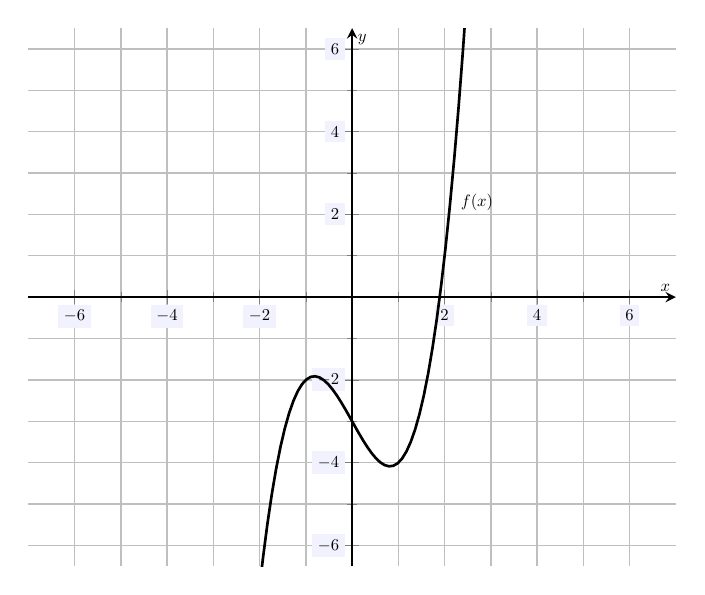
\begin{tikzpicture}[scale=1.2,every node/.style={scale=0.5}]
	\begin{axis}[
	grid=both,
	axis lines=middle,
	ticklabel style={fill=blue!5!white},
	xmin= -7, xmax=7,
	ymin= -6.5, ymax=6.5,
	xtick={-6,-4,-2,0,2,4,6},
	ytick={-6,-4,-2,0,2,4,6},
	minor tick = {-5,-3,...,5},
	xlabel=\(x\),ylabel=\(y\),
	samples=150
	]
	\node at (2.7,2.3) {$f(x)$};
	\addplot[thick,domain= -7:7] {x^3 - 2*x - 3};
	\end{axis}
	\end{tikzpicture}
	}
	\]

\begin{enumerate}[(a)]
\item What is $f(1)$? \pvspace{1.1cm}

{\itshape From the graph, we see that $f(1)= -4$.} \pvspace{1.1cm}


\item Is the point $(2, 1)$ on the graph of $f(x)$? Explain. \pvspace{1.1cm} 

{\itshape Because $f(x)$ passes through the point $(2, 1)$, the point $(2, 1)$ is on the graph of $f(x)$.} \pvspace{1.1cm}


\item Is the point $(-2, -2)$ on the graph of $f(x)$? Explain. \pvspace{1.1cm}

{\itshape We can see that $f(x)$ does not pass through the point $(-2, -2)$. Therefore, $(-2, -2)$ is not on the graph of $f(x)$.} \pvspace{0.5cm}


\item Is the function $f(x)$ even, odd, or neither. Explain. \pvspace{1.1cm}

{\itshape Because $f(x)$ is not symmetric across the $y$-axis and also not symmetric through the origin, $f(x)$ can be neither even nor odd.}
\end{enumerate}


%\printpoints
\end{document}